\documentclass{article}
\usepackage{graphicx}
\usepackage{subcaption}
\usepackage{float}
\usepackage{listings}
\usepackage{xcolor}
\usepackage{natbib}
\usepackage[utf8]{inputenc}   % Para usar acentuação direta no código
\usepackage[T1]{fontenc}      % Para melhorar a codificação das fontes
\usepackage[portuguese]{babel}    % Ou 'portuguese', mas 'brazil' é preferido

\author{Felipe B. R. Karmann, João M. S. da Silva e Souza}
\date{30 de junho de 2025}
\title{Uso de técnicas de processamento de imagem na identificação de alterações na cobertura vegetal em Blumenau}

\setlength{\oddsidemargin}{-0.5cm} % Margem esquerda
\setlength{\evensidemargin}{-0.5cm} % Margem direita (para documentos de duas páginas)
\setlength{\textwidth}{17cm} % Largura do texto
\setlength{\topmargin}{-1.5cm} % Margem superior
\setlength{\textheight}{24cm} % Altura do texto

\begin{document}

\maketitle

\section{Descrição do problema}

A cidade de Blumenau é historicamente vulnerável a enchentes, sendo este fato devido à sua geografia montanhosa, rios urbanos e padrões de chuva intensos. A gestão de riscos naturais requer ferramentas que combinem automação, visão computacional e análise de dados geográficos para monitorar o uso do solo e identificar áreas críticas.

A partir dos artigos escolhidos para servir de base para o nosso trabalho, o problema a ser resolvido é a criação de um programa que detecte padrões e características do terreno em fotos tiradas por satélites, e, usando técnicas de processamento de imagem, identifica alterações na cobertura vegetal de áreas que sofreram desastres naturais.

\section{Fonte dos dados}

A base de imagens foi criada com fotos de satélite da região de Blumenau obtidas no serviço Google Earth, com foco em áreas com grande cobertura vegetal. Para cada área selecionada, tiramos duas fotos, uma do dia 19 de abril de 2023 e outra do dia 17 de abril de 2025, tendo, portanto, quase exatamente dois anos de diferença. As fotos foram tiradas de uma altitude considerada por nós apropriada para a detecção de diferenças na cobertura vegetal.

A equipe tomou o devido cuidado para garantir que cada par de fotos tivesse a mesma posição no mapa para que não houvesse diferenças que não aquelas causadas pela passagem do tempo.

\section{O algoritmo}

O nosso programa pode ser dividido em quatro etapas básicas, cada uma consistindo numa técnica de processamento de imagens vista em sala de aula:
\begin{itemize}
  \item Segmentação (\texttt{MeanShift.py}): usamos o algoritmo Mean Shift para segmentar a imagem obtida em regiões de cores diferentes, tendo por base o valor médio da intensidade de cada região. Os resultados desta etapa se mostraram altamente precisos para a detecção de cobertura vegetal em áreas urbanas, uma vez que estas têm seu próprio esquema de cores facilmente distinguível de todo o resto (prédios, ruas, água, solo exposto, etc.). Esta etapa não é indispensável; a binarização sozinha é suficiente para destacar a vegetação em muitos casos, mas a segmentação ajuda a eliminar ruídos e sombras, garantindo assim um resultado mais preciso;
  \item Binarização (\texttt{Binarizar.py}): esta etapa se mostrou necessária por conta de diferenças que inevitavelmente existem entre duas fotos tiradas por satélite em momentos diferentes, normalmente relacionadas à hora do dia em que são tiradas, à qualidade da câmera usada ou à presença de filtros. Para normalizar o padrão de cores entre imagens, o algoritmo escolhe automaticamente o limiar usado na binarização calculando o nível médio de intensidade da imagem. Observamos que, invariavelmente, as áreas vegetais tornavam-se a parte escura da imagem, e todo o resto a parte clara;
  \item Subtração (\texttt{Subtrair.py}): em seguida, fazemos a subtração das duas imagens, cada uma representando o mesmo lugar em momentos diferentes;
  \item Erosão e dilatação (\texttt{Abertura.py}): agora, já obtivemos a diferença exata entre as duas imagens, representadas, no resultado da subtração, pelas regiões brancas. No entanto, devido à diferença que tende a existir entre duas imagens quaisquer, é provável que a maioria das regiões brancas representa não mais do que um pequeno acidente de fotografia, como uma sombra. Por isto, decidimos aplicar no final uma combinação de erosão e dilatação usando um elemento estruturante de tamanho 3 (também estudamos outros tamanhos, e o algoritmo pode ser ajustado conforme à necessidade). Desta maneira, regiões brancas insignificantes são eliminadas na erosão e não têm chance de retornar na dilatação, deixando apenas regiões significativas que possuem alto valor semântico para a análise de efeitos dos desastres naturais.
  \item Aplicação de máscaras (\texttt{AplicarMascara.py}): esta etapa pode ser vista como opcional; seu único propósito é facilitar a leitura do resultado. A partir do resultado da etapa anterior, as regiões brancas são transformadas em máscaras, que são em seguida aplicadas à imagem original para assinalar as regiões de interesse.
\end{itemize}

\section{Trechos de código}

Conforme mencionado anteriormente, nossa solução é dividida em quatro etapas básicas, que foram escritas cada uma em seu próprio arquivo; desta maneira, pudemos testar cada etapa do algoritmo separadamente. A entrada usada em cada arquivo era a saída gerada pela etapa anterior.

Começando pela parte que, do ponto de vista da codificação, foi a mais delicada, a Mean Shift (alguns trechos de código e linhas em branco foram removidos desta amostra para economizar espaço no documento):

\subsection{Mean Shift}

\begin{verbatim}
        array_imagem = np.array(imagem_original)
        altura, largura = array_imagem.shape[:2]
        imagem_plana = array_imagem.reshape((-1, 3))

        largura_banda = estimate_bandwidth(imagem_plana, quantile=quantil, n_samples=amostras)
        if largura_banda <= 0:
            largura_banda = 0.1

        print(f"Quantil usado: {quantil}, Largura de banda estimada: {largura_banda:.2f}")

        ms = MeanShift(bandwidth=largura_banda, bin_seeding=True)
        ms.fit(imagem_plana)
        rotulos = ms.labels_
        centros_cluster = ms.cluster_centers_
        num_clusters = len(np.unique(rotulos))

        imagem_segmentada = centros_cluster[rotulos].reshape(array_imagem.shape)
        imagem_segmentada = np.clip(imagem_segmentada, 0, 255).astype(np.uint8)

        imagem_resultante = Image.fromarray(imagem_segmentada)
        imagem_resultante.save(caminho_saida)

        return num_clusters
\end{verbatim}

O código acima é responsável por transformar a imagem em uma matriz plana de pixels, onde cada linha é um pixel com valores RGB, calcular o parâmetro de largura de banda para o Mean Shift e executar o seu algoritmo de segmentação nos pixels da imagem; cada pixel é atribuído a um cluster baseado em similaridade de cor. Finalmente, cada pixel é substiuído pelo centroide do seu cluster, resultando numa segmentação extremamente precisa e detalhada.

\subsection{Binarização}

\begin{verbatim}
    imagem = cv2.imread(caminho_imagem, cv2.IMREAD_GRAYSCALE)

    limiar = np.mean(imagem)
    print(f"Limiar automático calculado: {limiar:.2f}")
    _, imagem_binarizada = cv2.threshold(imagem, limiar, 255, cv2.THRESH_BINARY)
    cv2.imwrite(caminho_saida, imagem_binarizada)
    print(f"Imagem binarizada salva com sucesso em: {caminho_saida}")
\end{verbatim}

O algoritmo de binarização carrega a imagem em escala de cinza, calcula o limiar automaticamente como a média dos valores de intensidade dos pixels e aplica a binarização usando este limiar: pixels acima viram branco (255), abaixo viram preto (0).

\subsection{Subtração}

\begin{verbatim}
    imagem_diferenca = cv2.absdiff(imagem_antes, imagem_depois)
    imagem_diferenca_cinza = cv2.cvtColor(imagem_diferenca, cv2.COLOR_BGR2GRAY)
    _, imagem_binaria = cv2.threshold(imagem_diferenca_cinza, 50, 255, cv2.THRESH_BINARY)

    return imagem_diferenca, imagem_binaria
\end{verbatim}

O algoritmo de subtração calcula a diferença absoluta entre as duas imagens.

\subsection{Abertura}

\begin{verbatim}
    kernel = np.ones((kernel_size, kernel_size), np.uint8)

    img_filtrada = cv2.morphologyEx(img, cv2.MORPH_OPEN, kernel)

    cv2.imwrite(caminho_saida, img_filtrada)
    print(f"Imagem filtrada salva em: {caminho_saida} (Kernel = {kernel_size}x{kernel_size})")
\end{verbatim}

O algoritmo de erosão e dilatação utiliza um elemento estruturante (ou kernel) de tamanho 3 e aplica a operação de abertura morfológica, erosão seguida de dilatação. Esta operação remove pequenos regiões brancas enquanto mantém as principais, conforme explicado na seção anterior.

\subsection{Aplicação de máscaras}

\begin{verbatim}
    resultado = imagem.copy()
    for mascara in mascaras:
        regiao_mascarada = cv2.bitwise_and(imagem, imagem, mask=mascara)
        hsv = cv2.cvtColor(regiao_mascarada, cv2.COLOR_BGR2HSV)
        hsv[:,:,1] = 255  # Saturação máxima
        hsv[:,:,2] = np.where(mascara > 0, 255, hsv[:,:,2])  # Valor máximo nas áreas mascaradas
        regiao_saturada = cv2.cvtColor(hsv, cv2.COLOR_HSV2BGR)
        resultado = cv2.addWeighted(resultado, 1, regiao_saturada, 0.7, 0)
    return resultado
\end{verbatim}

O algoritmo de aplicação de máscaras retorna uma nova imagem onde as áreas definidas pelas máscaras foram realçadas visualmente, com cores mais saturadas e brilho máximo. As outras regiões permanecem inalteradas.

\section{Exemplo de resultados}

Para esta demonstração, usaremos duas imagens da região central de Blumenau, uma de 2023 e outra de 2025:

\begin{figure}[H]
    \centering
    \begin{subfigure}[b]{0.48\textwidth}
        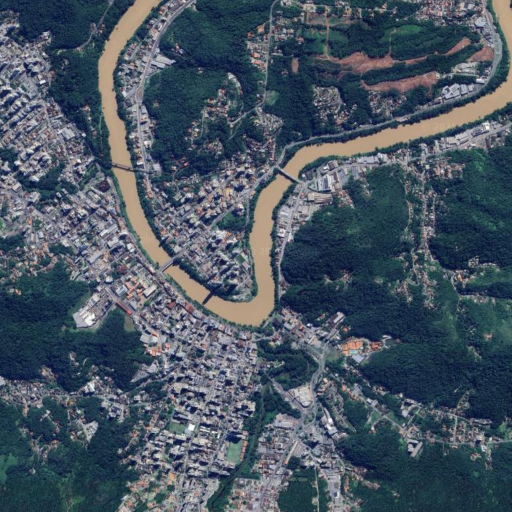
\includegraphics[width=\textwidth]{../Imagens/012023.png}
        \caption{O centro de Blumenau em 2023.}
        \label{2023}
    \end{subfigure}
    \hfill % Espaço entre as imagens
    \begin{subfigure}[b]{0.48\textwidth}
        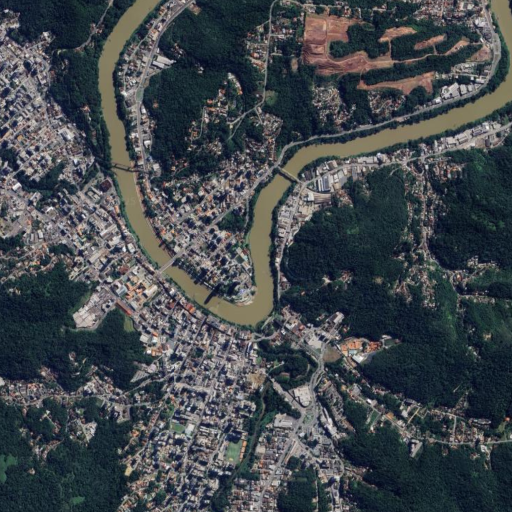
\includegraphics[width=\textwidth]{../Imagens/012025.png}
        \caption{O centro de Blumenau em 2025.}
        \label{2025}
    \end{subfigure}
    \caption{As fotos originais.}
    \label{original}
\end{figure}

Como é fácil notar, as imagens possuem diferença significativa no nível de intensidade. Nós atribuímos a causa provável disto à hora do dia e às condições de iluminação natural.

Conforme explicado anteriormente, o próximo passo é a clusterização das imagens usando o algoritmo Mean Shift:

\begin{figure}[H]
    \centering
    \begin{subfigure}[b]{0.48\textwidth}
        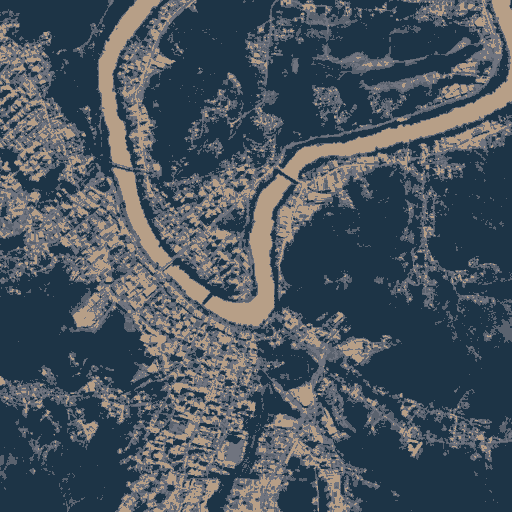
\includegraphics[width=\textwidth]{../Imagens/012023_mean_shift.png}
        \caption{A foto de 2023 segmentada.}
        \label{2023}
    \end{subfigure}
    \hfill % Espaço entre as imagens
    \begin{subfigure}[b]{0.48\textwidth}
        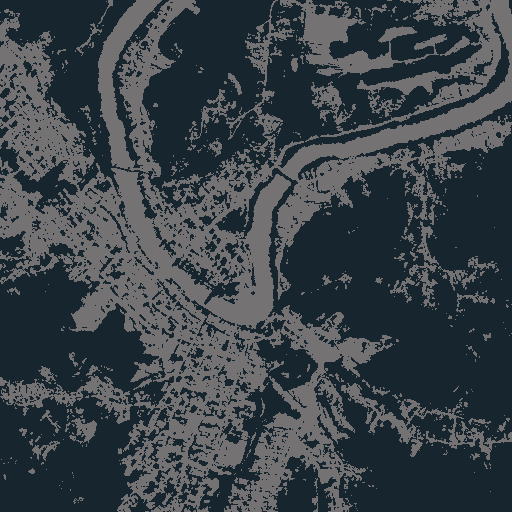
\includegraphics[width=\textwidth]{../Imagens/012025_mean_shift.png}
        \caption{A foto de 2025 segmentada.}
        \label{2025}
    \end{subfigure}
    \caption{Resultado da aplicação do Mean Shift.}
    \label{segmentada}
\end{figure}

Vale notar que a segmentação da imagem de 2023 assinalou muitas pequenas regiões da cidade com a mesma cor que a água do rio. Isto não será um problema; o algoritmo de binarização destacará a porção vegetal de todas as regiões mais claras:

\begin{figure}[H]
    \centering
    \begin{subfigure}[b]{0.48\textwidth}
        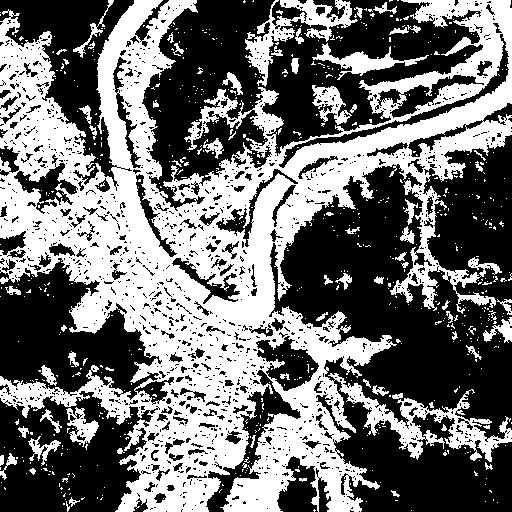
\includegraphics[width=\textwidth]{../Imagens/012023_bin.png}
        \caption{A foto de 2023 binarizada.}
        \label{2023}
    \end{subfigure}
    \hfill % Espaço entre as imagens
    \begin{subfigure}[b]{0.48\textwidth}
        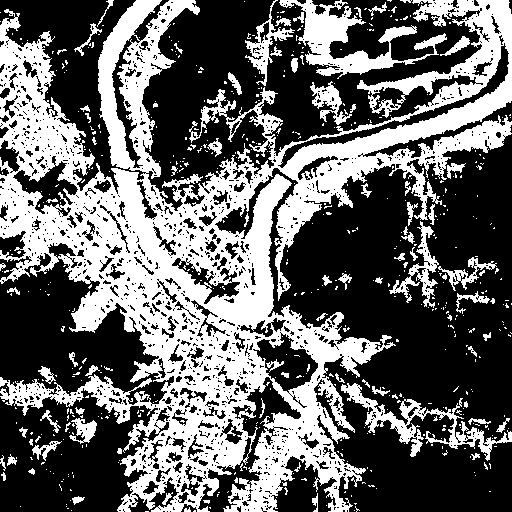
\includegraphics[width=\textwidth]{../Imagens/012025_bin.png}
        \caption{A foto de 2025 binarizada.}
        \label{2025}
    \end{subfigure}
    \caption{Resultado da binarização.}
    \label{binarizada}
\end{figure}

Finalmente, é o momento de fazer a subtração das duas imagens para apontar diferenças na cobertura vegetal entre estes dois anos. Como explicado anteriormente, há a presença de muitas pequenas regiões claras no resultado, o que por sua vez resulta em parte da diferença de intensidade entre as duas imagens e noutra parte de fatores não naturais (corte intencional de árvores, por exemplo). Por este motivo, aplicamos o algoritmo de erosão e dilatação para eliminar diferenças consideradas insignificantes. Abaixo o resultado:

\begin{figure}[H]
    \centering
    \begin{subfigure}[b]{0.48\textwidth}
        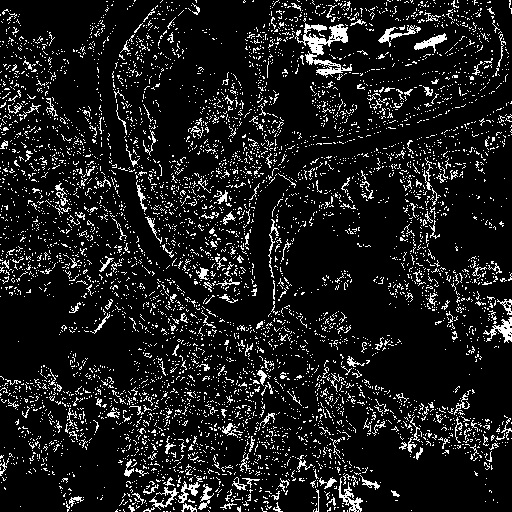
\includegraphics[width=\textwidth]{../Imagens/012025_sub.png}
        \caption{O resultado da subtração das imagens.}
        \label{2023}
    \end{subfigure}
    \hfill % Espaço entre as imagens
    \begin{subfigure}[b]{0.48\textwidth}
        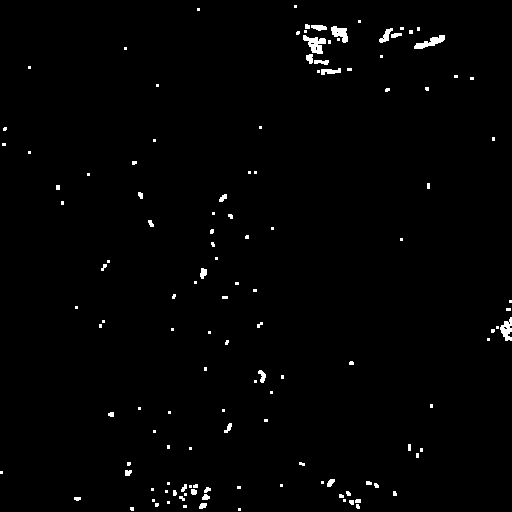
\includegraphics[width=\textwidth]{../Imagens/resultado01.png}
        \caption{A imagem ao lado após a erosão e a dilatação.}
        \label{2025}
    \end{subfigure}
    \caption{Isolando regiões de interesse.}
    \label{resultado}
\end{figure}

A partir da última figura, podemos observar que a maior área de interesse está na região norte da imagem. Conferindo nas imagens originais, é possível verificar que houve, entre 2023 e 2025, um aumento significativo na porção de solo exposto naquela região, em prejuízo da cobertura vegetal.

\begin{figure}[H]
    \centering
    \begin{subfigure}[b]{0.48\textwidth}
        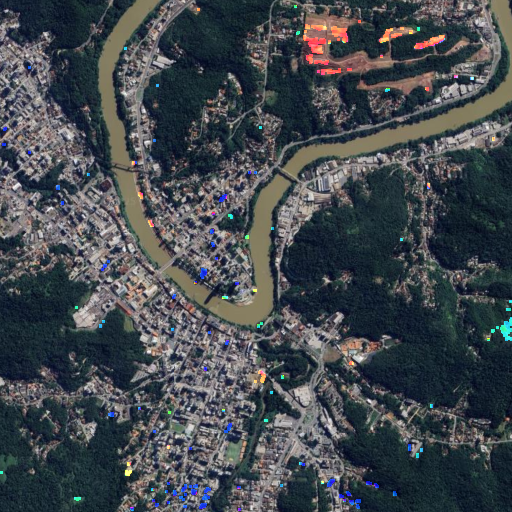
\includegraphics[width=\textwidth]{../Imagens/resultado01_mask.png}
        \caption{A máscara isolada.}
        \label{2025}
    \end{subfigure}
    \hfill % Espaço entre as imagens
    \begin{subfigure}[b]{0.48\textwidth}
        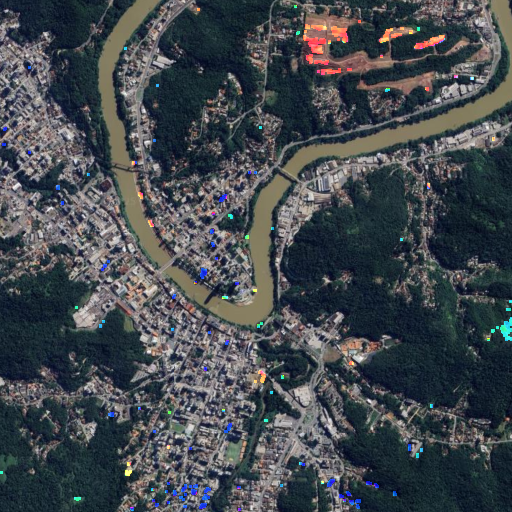
\includegraphics[width=\textwidth]{../Imagens/012025_mask.png}
        \caption{A máscara aplicada à foto de 2025.}
        \label{2025}
    \end{subfigure}
    \caption{O resultado da aplicação das máscaras.}
    \label{máscara}
\end{figure}

Gerando e aplicando máscaras a partir da imagem binarizada e aberta, a correspondência das regiões fica mais evidente. Observa-se que o contraste com o fundo marrom do solo exposto, somado ao efeito de transparência da máscara, lhe confere um tom vermelho, o que também serve para indicar a principal região de interesse.

\nocite{*}
\bibliographystyle{plain}
\bibliography{referencias}

\end{document}
